\section{Learning which equations to construct after seed tuning}
\label{sec:equation-refinement}
The seed-bound experiment shows that tuning a fixed configuration explains most of its time saving. We therefore keep those tuned seed limits and train a model for a finer decision: whether to construct each equation inside the selected region. This comparison asks whether learned equation selection supplies an additional saving after the coarse seed region has already been improved.

\subsection{Model and integration with exact reduction}
Each candidate consists of a seed integral and one IBP or Lorentz-invariance operator. A classification tree uses the seventeen quantities in Table~\ref{tab:refinement-features}, including seed powers, target powers, distance to a target, and operator index. All these quantities are available before symbolic coefficient construction. The tree follows feature-threshold tests to a terminal node, called a leaf. The leaf score is the weighted positive fraction of its training examples, and Kira constructs the equation when that score meets the selected threshold. We also test a learned seed choice that retains every operator from a seed when at least one operator receives a score above the threshold. This uses the same trained scores and keeps more identities from each retained seed, which can prevent a failed reduction. Validation compares both uses of the model. Native symmetries, exact elimination, and back substitution remain in use. A failed attempt triggers the same tuned seed configuration with the filter disabled, followed by native and expanded bounds if needed. Thus the reported cost includes the consequences of an insufficient equation set.

The training label records whether the equation's integral support appears in Kira's final selected system. Support means the set of integrals with nonzero coefficients. This label is a proxy for usefulness and does not identify a unique necessary equation set. We collect new labels with the tuned seed settings because changing those settings changes which equations Kira can select. Collection uses a Kira build that records selected supports, and every collected reduction must agree with the independent exact reference. The timed comparisons use the same current build for both methods. The earlier filters frequently need a complete retry on these inputs, so their previous performance does not justify using them without new validation.

The four-loop box with bubbles has no completed label collection within the resource allowance, so it uses unfiltered reduction in this test. We preserve those collection failures. For the nine remaining structures, we fit eight shared classification trees and eight separate trees per graph~\cite{CART1984,Pedregosa2011Bounds}, with maximum depths 6, 10, 14, or 18 and minimum leaf populations 4 or 16, and a limit of 4,096 leaves. The data contain 137015 sampled equation records, including 39285 positive labels, from 66 training batches. Sampling weights preserve the native class proportions and give each batch equal total weight. The model receives no final reduction coefficients. Validation uses 33 separate batches, first to find filters that retain nearly all positive labels and then to measure complete reduction cost. A graph uses a learned seed or equation filter only when its median validation cost is at least 5\% below the same tuned calculation with all ML disabled. Appendix~\ref{app:equation-refinement} specifies the fitting, threshold selection, and recovery rules.

\subsection{Reserved comparison and the additional learned gain}
We freeze the trees, thresholds, graph choices, and domain limits before evaluating two new rational kinematic profiles, $h=525,526$. The dimension remains symbolic. The ten graph structures and target patterns are the same as in Appendix~\ref{app:learned-bounds}; the new profiles supply distinct kinematic requests. Some index patterns repeat training patterns, including the planar and nonplanar boxes at these two profiles. This is a test within known structures at one through four loops. A separate comparison below changes the target-index batches as well. As in the seed-bound study, each timed request receives a common master basis, and independent reference coefficients enter only the final exact comparison.

Both methods use the same executable, tuned seed limits, native row choices, exact implementation improvements, worker count, and recovery limits. The control disables every learned selector. Five repetitions alternate the order of the two methods. Time includes policy loading, the domain check, equation prediction and generation, exact algebra, verification, retries, and cleanup. Initial Python imports and construction of the common reference basis remain outside this repeated timer. A domain check disables filtering for an unrecognized ordered graph or target complexity outside the saved ranges.

The reserved grid has 74 requests. It supplies 68 matched nontrivial batches, with 4 failed reference checks, 0 incomplete timed batches, and 2 identity-only batches kept separately. All successful outputs pass exact coefficient comparisons: 700 completions among 700 timed requests, with 15430 comparisons. Table~\ref{tab:equation-refinement} retains each graph, including any slower result.

\begin{table}[!htbp]\centering\small
\caption{Additional effect of the equation model after fixed seed tuning. Times are sums of batch medians in seconds. ``Active'' counts batches on which the frozen policy enables filtering. A ratio below one means less complete time.}
\label{tab:equation-refinement}
\begin{tabular}{@{}lrrrrrr@{}}\toprule
Graph & Loops & Batches & Active & ML off & Policy & Ratio\\\midrule
Massive sunrise & 2 & 8 & 0 & 4.70 & 4.69 & 0.997\\
Planar double box & 2 & 8 & 8 & 18.78 & 15.79 & 0.841\\
Massive vacuum & 3 & 8 & 8 & 8.07 & 7.55 & 0.937\\
Massive three-loop ladder & 3 & 8 & 8 & 26.12 & 23.97 & 0.918\\
Nonplanar box & 2 & 8 & 8 & 38.74 & 37.07 & 0.957\\
Pentagon & 1 & 8 & 0 & 6.75 & 6.64 & 0.983\\
Box with virtual leg & 1 & 8 & 0 & 4.85 & 4.83 & 0.996\\
Box with bubbles, 3 loops & 3 & 6 & 0 & 9.48 & 9.50 & 1.002\\
Box with bubbles, 4 loops & 4 & 2 & 0 & 30.99 & 31.16 & 1.005\\
Massless two-point, 4 loops & 4 & 4 & 0 & 5.44 & 5.38 & 0.990\\
\bottomrule\end{tabular}
\end{table}

The full matched workload changes from 153.937 to 146.586 seconds, a time saving of 4.8\%. For the 32 batches on which the frozen policy enables a filter, the corresponding times are 91.707 and 84.384 seconds, giving 8.0\% less time. The 95\% intervals from resampling paired repetitions are $[0.946, 0.959]$ for the full workload ratio and $[0.916, 0.927]$ for the active subset. The active subset follows the pre-test policy and is not selected from the observed test speedups. These intervals describe timing variation on the tested requests, not generalization to arbitrary graphs.

\begin{figure}[!htbp]\centering
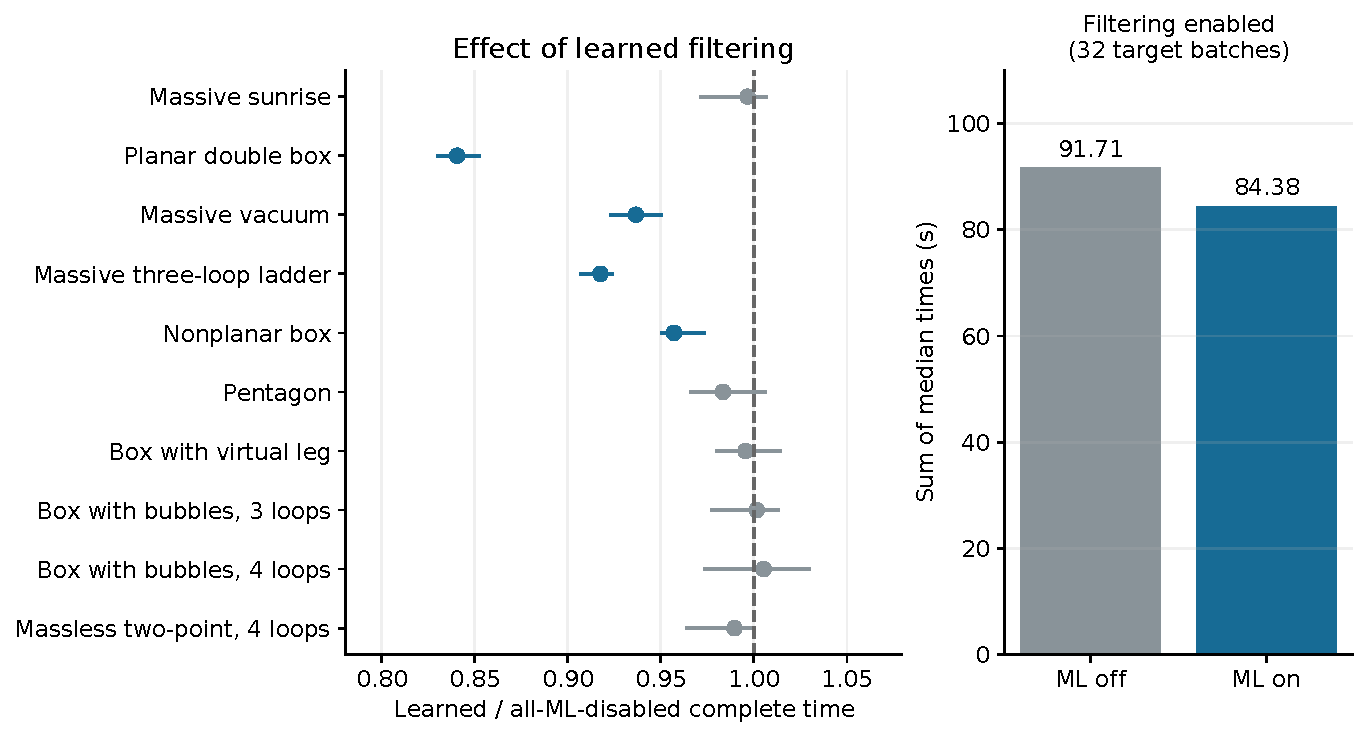
\includegraphics[width=\linewidth]{paper_figures/equation_refinement_times.pdf}
\caption{The left panel shows the complete-time ratio for every matched graph. Blue marks graphs with filtering enabled; grey marks graphs using the unchanged exact calculation. Horizontal intervals show the 95\% range from resampling paired repetitions within each graph. The right panel isolates the batches on which the preselected policy uses the trained filter. The control shares all exact optimizations and tuned seed settings, so the difference includes only the learned policy and its consequences.}
\label{fig:equation-refinement}
\end{figure}

On active requests, the filters reject 36.8\% of candidate construction calls, with a mean recorded filtering cost of 16.972 milliseconds per request. Repeated generation passes contribute to this count. Recovery can construct some rejected equations later, and its full cost remains in the timing comparison. The learned policy makes 5 recovery attempts in the reserved comparison. Recorded development, label collection, validation, and fitting take 39.2 minutes, excluding earlier seed-tuning costs. This expense precedes application and must be recovered over repeated use. A useful model on this collection does not establish a benefit for an unsupported topology, symbolic kinematics beyond the dimension, or all high-loop integrals. The separate wider coverage results retain their stated scope.

\subsection{Complete application launches}
A separate check starts a fresh application process for each request and supplies only the target definition and master basis. It uses the first supported reserved request for each graph where validation enabled filtering, with three rotated repetitions. These are a subset of the same reserved physical inputs. The timer includes Python startup, input parsing, model loading, output storage, process exit, and the exact coefficient check. Across 4 matched requests, summed median time changes from 21.835 seconds with all ML disabled to 18.946 seconds with the filter, giving a time saving of 13.2\%. This comparison checks the live application overhead; it does not add new graph structures to the physical scope.

\subsection{Transfer to new target-index batches}
The primary comparison changes kinematics but partly repeats the index patterns seen in training. To test index transfer separately, we keep the original fitted models, thresholds, and graph choices and define profiles $h=605,606$. We retain a batch only if its set of index vectors is absent from both training and validation and contains at least one individual index vector absent from those sets. We also remove repeated batches within each profile. These conditions select inputs from the graph structures enabled by the original validation; no primary test timing enters this selection. The selection rules and all resulting inputs are fixed before their reductions begin. The test therefore changes the indices within known graph structures and degree ranges, while transfer to new topologies remains untested.

Each request receives the same reference reduction and enlarged-region check as the primary comparison. Three repetitions rotate the two methods. The live application reads only a target definition and a master basis. Time includes basis reading, policy loading, prediction, exact reduction, recovery, and coefficient checks; it excludes initial Python imports and reference construction. Both methods retain the same seed settings and exact implementation.

\begin{table}[!htbp]\centering\small
\caption{The unchanged learned policy on new index batches. Times are sums of batch medians in seconds. The control disables every learned selector.}
\label{tab:index-transfer}
\begin{tabular}{@{}lrrrr@{}}\toprule
Graph & Batches & ML off & Policy & Ratio\\\midrule
Planar double box & 6 & 14.644 & 14.614 & 0.998\\
Massive three-loop ladder & 6 & 21.815 & 19.833 & 0.909\\
Nonplanar box & 6 & 29.771 & 27.317 & 0.918\\
Massive vacuum & 6 & 6.066 & 5.714 & 0.942\\
\bottomrule\end{tabular}
\end{table}

The structural rule defines 24 requests, of which 24 give matched nontrivial reductions. The record retains 0 failed reference checks, 0 incomplete comparisons, and 0 identity-only batches. All 144 successful outputs among 144 timed requests pass exact comparison, with 5106 coefficient checks. The summed median time changes from 72.295 to 67.478 seconds, giving 6.7\% less time. The 95\% paired-repetition interval for the learned-to-control ratio is $[0.928, 0.940]$. Table~\ref{tab:index-transfer} retains every matched graph, including any slower result. This check provides separate evidence about changes in target indices and is not combined with the primary timings to form a cumulative speedup.
